\documentclass[11pt]{article}

% Preamble

\usepackage[margin=1in]{geometry}
\usepackage{amsfonts, amsmath, amssymb}
\usepackage{fancyhdr, float, graphicx}
\usepackage[utf8]{inputenc} % Required for inputting international characters
\usepackage[T1]{fontenc} % Output font encoding for international characters
\usepackage{fouriernc} % Use the New Century Schoolbook font
\usepackage[nottoc, notlot, notlof]{tocbibind}
\usepackage{listings}
\usepackage{xcolor}
\usepackage{karnaugh-map}
% \usepackage[table,xcdraw]{xcolor}

\definecolor{codegreen}{rgb}{0,0.6,0}
\definecolor{codegray}{rgb}{0.5,0.5,0.5}
\definecolor{codepurple}{rgb}{0.58,0,0.82}
\definecolor{backcolour}{rgb}{0.95,0.95,0.92}

\lstdefinestyle{mystyle}{
    backgroundcolor=\color{backcolour},   
    commentstyle=\color{codegreen},
    keywordstyle=\color{magenta},
    numberstyle=\tiny\color{codegray},
    stringstyle=\color{codepurple},
    basicstyle=\ttfamily\footnotesize,
    breakatwhitespace=false,         
    breaklines=true,                 
    captionpos=b,                    
    keepspaces=true,                 
    numbers=left,                    
    numbersep=5pt,                  
    showspaces=false,                
    showstringspaces=false,
    showtabs=false,                  
    tabsize=2
}

\lstset{style=mystyle}

% Header and Footer
\pagestyle{fancy}
\fancyhead{}
\fancyfoot{}
\fancyhead[L]{\textit{\Large{DECA Assignment 5}}}
%\fancyhead[R]{\textit{something}}
\fancyfoot[C]{\thepage}
\renewcommand{\footrulewidth}{1pt}



% Other Doc Editing
% \parindent 0ex
%\renewcommand{\baselinestretch}{1.5}

\begin{document}

\begin{titlepage}
	\centering

	%---------------------------NAMES-------------------------------

	\huge\textsc{
		MIT World Peace University
	}\\

	\vspace{0.75\baselineskip} % space after Uni Name

	\LARGE{
		Digital Electronics and Computer Architecture\\
		Second Year B. Tech, Semester 3
	}

	\vfill % space after Sub Name

	%--------------------------TITLE-------------------------------

	\rule{\textwidth}{1.6pt}\vspace*{-\baselineskip}\vspace*{2pt}
	\rule{\textwidth}{0.6pt}
	\vspace{0.75\baselineskip} % Whitespace above the title



	\huge{\textsc{
		3 bit Synchronous UP Counter using JK- Flip flop 
		}} \\



	\vspace{0.5\baselineskip} % Whitespace below the title
	\rule{\textwidth}{0.6pt}\vspace*{-\baselineskip}\vspace*{2.8pt}
	\rule{\textwidth}{1.6pt}

	\vspace{1\baselineskip} % Whitespace after the title block

	%--------------------------SUBTITLE --------------------------	

	\LARGE\textsc{
		Practical Report\\
		Assignment 5
	} % Subtitle or further description
	\vfill

	%--------------------------AUTHOR-------------------------------

	\vspace{0.5\baselineskip} % Whitespace before the editors

	\Large{
		Krishnaraj Thadesar \\
		Cyber Security and Forensics\\
		Batch A2, PA 34
	}


	\vspace{0.5\baselineskip} % Whitespace below the editor list
	\today

\end{titlepage}


\tableofcontents
\thispagestyle{empty}
\clearpage


\setcounter{page}{1}
\section{Objectives}
\begin{enumerate}
	\item To understand the operation of Synchronous counter
	\item To design and implement 3-Bit Synchronous UP counter using JK- Flip flop
	
\end{enumerate}

\section{Problem Statement}
Design and Implement 3 bit Synchronous UP Counter using JK- Flip flop 

\section{ICs Used}

\begin{enumerate}
	\item IC7408 (AND Gate)
	\item IC7476 (Dual Master Slave JK Flip Flop)
\end{enumerate}

\section{Platform Used}
Digital Trainer Kit

\section{Theory}
\subsection{Definition of Synchronous counter}
Synchrounous generally refers to something which is cordinated with others based on time. Synchronous signals occur at same clock rate and all the clocks follow the same reference clock.\\

In previous tutorial of Asynchronous Counter, we have seen that the output of that counter is directly connected to the input of next subsequent counter and making a chain system, and due to this chain system propagation delay appears during counting stage and create counting delays. In synchronous counter, the clock input across all the flip-flops use the same source and create the same clock signal at the same time. So, a counter which is using the same clock signal from the same source at the same time is called Synchronous counter.

\subsection{Advantages of Synchronous counter}

\begin{enumerate}
	\item It’s easier to design than the Asynchronous counter.
	\item It acts simultaneously.
	\item No propagation delay associated with it.
	\item Count sequence is controlled using logic gates, error chances are lower.
	\item Faster operation than the Asynchronous counter.
\end{enumerate}

\subsection{Application of Synchronous counter}
\begin{enumerate}
	\item Machine Motion control
	\item Motor RPM counter
	\item Rotary Shaft Encoders
	\item Digital clock or pulse generators.
	\item Digital Watch and Alarm systems.
\end{enumerate}

\subsection{Involved Truth Tables}

\subsubsection{AND Gate}

\begin{table}[H]
	\begin{tabular}{|c|c|c|}
		\hline
		{\color[HTML]{000000} \textbf{A}} & {\color[HTML]{000000} \textbf{B}} & {\color[HTML]{000000} \textbf{Q}} \\ \hline
		{\color[HTML]{330001} \textit{0}} & {\color[HTML]{330001} \textit{0}} & {\color[HTML]{F56B00} \textit{0}} \\ \hline
		{\color[HTML]{330001} \textit{0}} & {\color[HTML]{330001} \textit{1}} & {\color[HTML]{F56B00} \textit{1}} \\ \hline
		{\color[HTML]{330001} \textit{1}} & {\color[HTML]{330001} \textit{0}} & {\color[HTML]{F56B00} \textit{1}} \\ \hline
		{\color[HTML]{330001} \textit{1}} & {\color[HTML]{330001} \textit{1}} & {\color[HTML]{F56B00} \textit{1}} \\ \hline
	\end{tabular}
\end{table}

\subsubsection{Truth table of 3 Bit synchrounous down counter. }

\subsubsection{Function Table of the IC7476}
\begin{figure}[H]
	\centering
	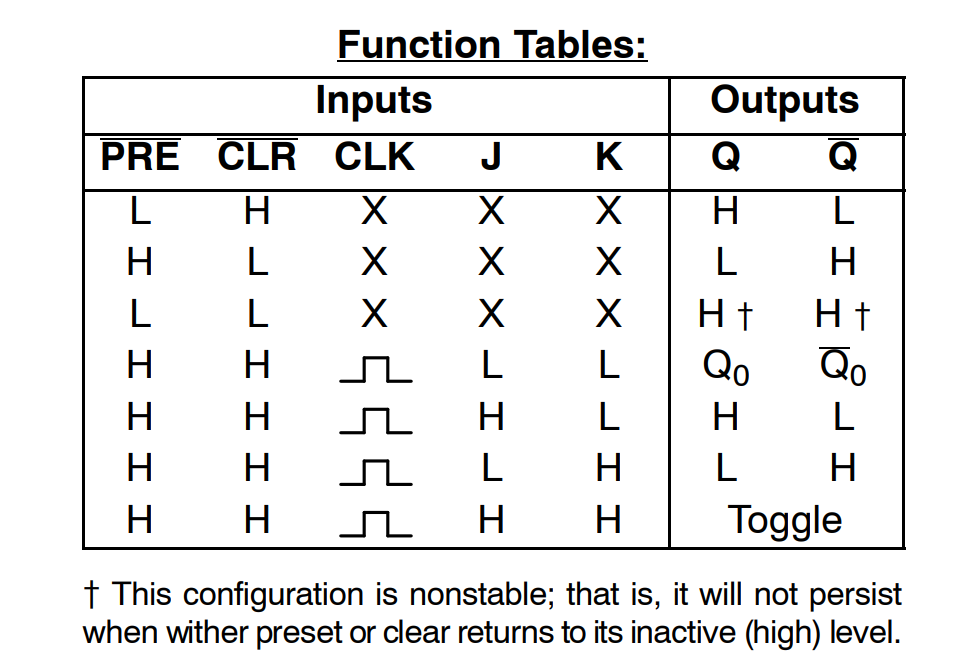
\includegraphics[scale = 0.5]{7476 function table.png}
	\caption{Function Table for IC 7476}
\end{figure}

\subsection{JK Flip Flop Truth table}
\begin{figure}[H]
	\centering
	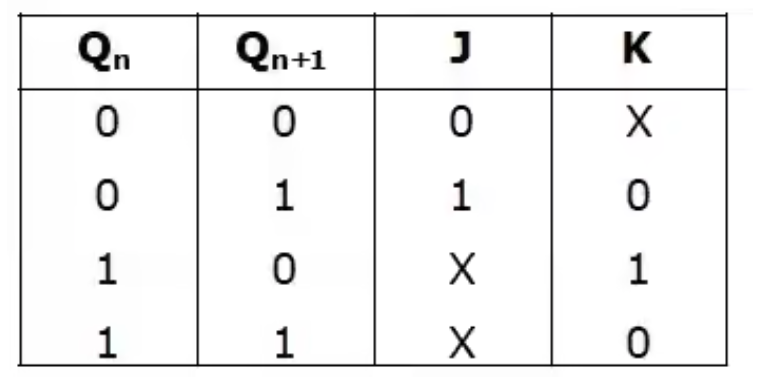
\includegraphics[scale = 0.4]{jk flip flop truth table.png}
	% \caption{Circuit diagram of a 3-bit synchronous counter - Down}
\end{figure}
\subsection{JK Flip Flop Excitation table}
\begin{figure}[H]
	\centering
	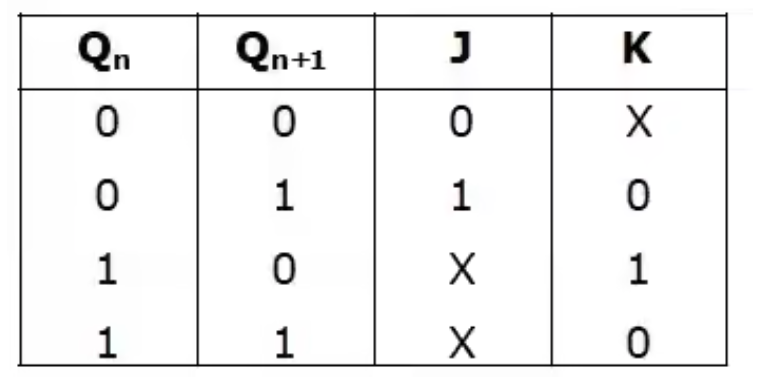
\includegraphics[scale = 0.4]{jk flip flop excitation table.png}
	% \caption{Circuit diagram of a 3-bit synchronous counter - Down}
\end{figure}
\subsection{JK Flip Flop Characteristic table}
\begin{figure}[H]
	\centering
	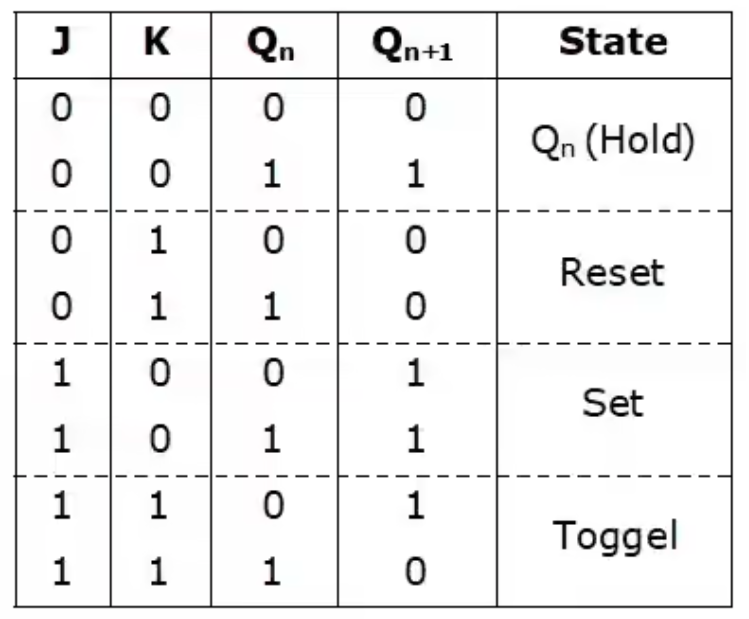
\includegraphics[scale = 0.4]{jk flip flop characteristic table.png}
	% \caption{Circuit diagram of a 3-bit synchronous counter - Down}
\end{figure}

\subsection{State diagram of 3 Bit Synchronous Down Counter}

\begin{figure}[H]
	\centering
	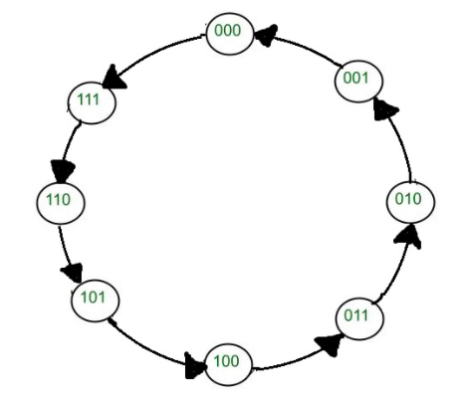
\includegraphics[width=0.45\textwidth]{state diagram 3 bit synchronous.png}
	\label{fig:}
\end{figure}


\section{Pin Diagrams of ICs Used}

\subsection{Pin Diagram of IC7476}
\begin{figure}[H]
	\centering
	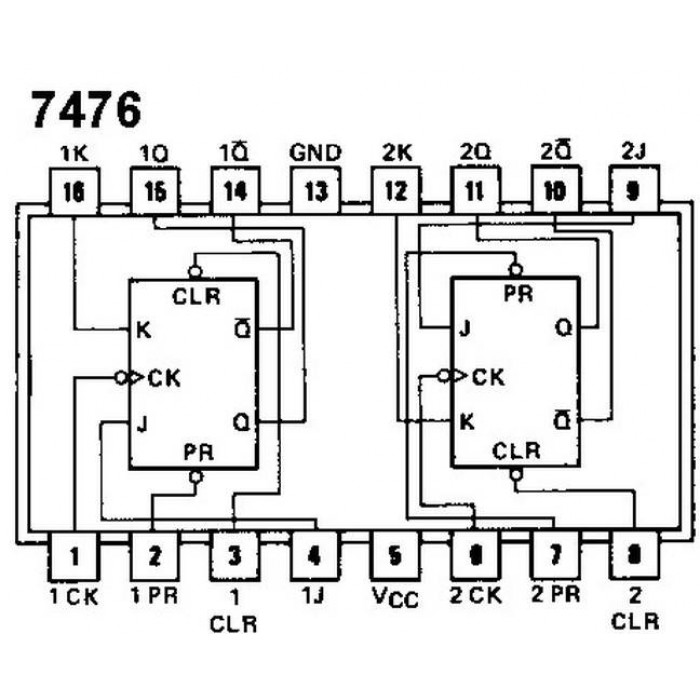
\includegraphics[scale = 0.35]{7476.jpg}
	\caption{Pin Diagram for IC 7476}
\end{figure}
\subsection{Pin Diagram of IC7408}
\begin{figure}[H]
	\centering
	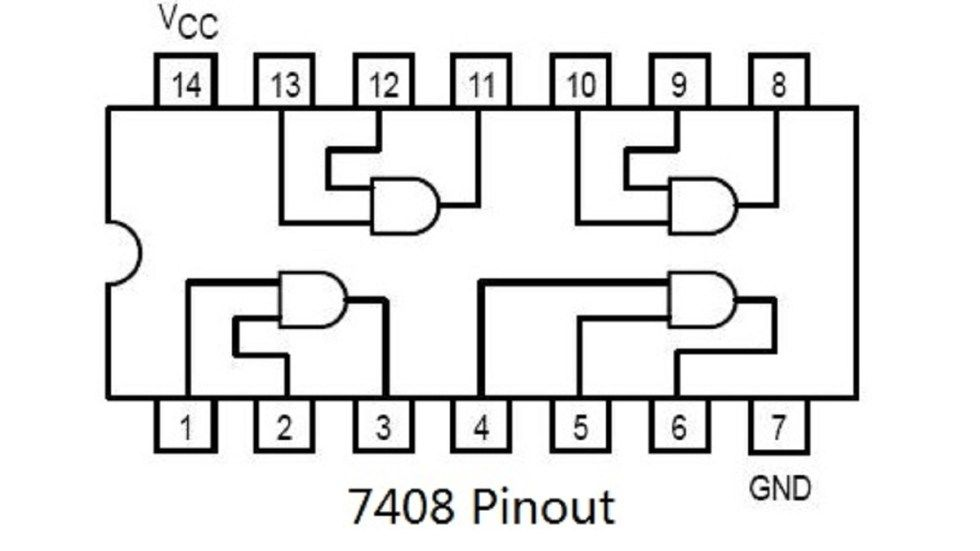
\includegraphics[scale = 0.25]{7408.jpg}
	\caption{Pin Diagram for IC 7408}
\end{figure}

\section{Design and Implementation}

\subsection{Circuit diagram of a 3-bit asynchronous counter: (3 Bit Asynchronous - DOWN Counter / Modulus 8)}

\begin{figure}[H]
	\centering
	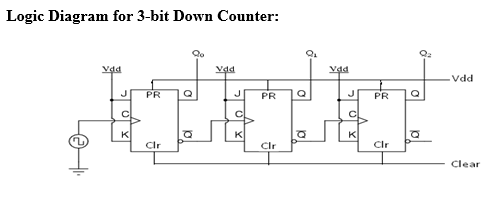
\includegraphics[scale = 1.4]{bit synch down counter.png}
	\caption{Circuit diagram of a 3-bit synchronous counter - Down}
\end{figure}


\section{Procedure}

\begin{enumerate}
	\item Design Sequential circuit logic circuit as per given problem statement.
	\item Connect the IC 74LS76 and other basic logic gate ICs as per diagram.
	\item Give VCC supply and ground connection to each IC.
	\item Give clock to first JK FF.
	\item Observe the output and verify the truth table.
	\item Switch off the power supply of trainer kit.
\end{enumerate}

\section{Conclusion}
\textit{Thus, we have learnt a fundamental application and working of the IC 7476, and verified the truth table of its dual Master Slave JK Flip Flops. The Logic of Flip Flops was understood in detail, and implemented on the Digital Trainer Kit. Synchronous counters were also implemented with MOD 8. Their results were observed, noted and understood. }
\pagebreak

\section{FAQs}

\begin{enumerate}
	\item Why a synchronous counter operate at a higher frequency than a ripple counter? \\
	
	Synchronous counters can operate at a higher frequency than a ripple counter because the dual flip flops in the counter operate at the same time, therefore reducing the time by a huge margin, and subsequently increasing the frequency. 
	\item A 5-bit synchronous binary counter is made up of five flip-flops, each with a 12 ns propagation delay. The total propagation delay (tp(total)) is ?\\

	Each bit has propagation delay = 12ns. So, 5 bits = 12ns * 5 = 60ns. Since a counter is constructed using flip-flops, therefore, the propagation delay in the counter occurs only due to the flip-flops. Each bit has propagation delay = 15ns.
	


	
\end{enumerate}

\end{document}